\chapter{Experiment}
In the last chapter we discussed about the design of MPLS Opportunistic Security. In this chapter I will be explaining the implementation of MPLS OS in the OpenVSwitch Kernel

\section{Infrastructure setup}

The project is implemented in OpenVSwitch kernel. OpenVSwitch is a linux open flow technology which can be installed in Linux machines. All flavours of Linux are supported with OpenVSwitch.\\  

In order to emulate the MPLS Switches and Hosts, either we can install containers in the Linux. Each container can act as an OpenVswitch. Interconnect 2 containers as 2 LSRs connected each other.\\ 

There is an additional overhead when we use multiple containers in the same Linux machine as the kernel crashed many times and the latency collected during the test was unreliable. Hence the implementation further conducted in mininet.\\ 

The topology diagram is given in the figure 3.1. The testing of the final implementation is carried out by sending an icmp ping packet from Host H1 to Host H3.
\subsection{Setting up Mininet}

Mininet can be downloaded and installed in using the command sudo apt-get install mininet. This will install both mininet and openvswitch. The problem is we cannot edit the openvswitch kernel (OVSK) of the openvswitch installed along with the openvswitch. 

To check the working of mininet, we can setup a simple topology of 1 switch and 2 host and ping from both the host using the command sudo mn --test pingall. 

To setup the topology of our experiment, we can use the command sudo mn –topo=linear,3 –switch=ovsk –controller=ovsc 

 
This will initiate 3 switches with one host on each and the switches will be connected serially as shown in the figure 3.1. 

The parameters in the mininet initiation command is given below. 

topo=linear,3: This is for initiating 3 switches with 1 host each and connect the switches linearly. 

–switch=ovsk: This is for using openvswitch kernel as the switch kernel 

–controller=ovsc: This is for choosing openvswitch controller as the openflow SDN controller. 
\subsection{Setting up OpenVswitch}

Installing mininet will install OpenVswitch too. However we cannot edit the kernel of the openvswitch installed along with mininet. We have to install OpenVswitch with version of our choice and then replace the openvswitch installed by mininet from the kernel. 

We can see the module informsation using the command lsmod in the linux.  

We can download the Openvswitch using git clone. The link for downloading is  

git clone https://github.com/openvswitch/ovs.git. Once downloaded we have to bootstrap the image using the script boot.sh in the package and after that we have to configure it using the script configure. Inorder to build the package we have to run the following commands, 



\subsubsection{make} 
\subsubsection{make install}
\subsubsection{make modules_install"}
\subsubsection{/sbin/modprobe openvswitch}\\



Inorder to start the openvswitch, use the following commands,\\

\subsubsection{export PATH=$PATH:/usr/local/share/openvswitch/scripts} 

\subsubsection{ovs-ctl start} 

 \section{Testing the MPLS System}
 
 \subsection{Addition of the MPLS flows}

In order to test the working of MPLS, we have to add MPLS flows to the openvwitch. The topology can be initiated using the command\\ sudo mn –topo=linear,3 –switch=ovsk –controller=ovsc. 

Once the topology is initiated, we can add mpls flows to each OVS Switch using the commands given below. \\

To install mpls flow from S1 to S3 through S2 \\

sudo ovs-ofctl -O OpenFlow13 add-flow s1 "table=0,in_port=1,eth_type=0x800,actions=goto_table:1" 

sudo ovs-ofctl -O OpenFlow13 add-flow s1 "table=1,in_port=1,eth_type=0x800,actions=push_mpls:0x8847,set_field:12->mpls_label,output:2" 

sudo ovs-ofctl -O OpenFlow13 add-flow s2 "table=0,in_port=2,eth_type=0x8847,actions=output:3" 

sudo ovs-ofctl -O OpenFlow13 add-flow s3 "table=0,in_port=2,eth_type=0x8847,actions=goto_table:1" 

sudo ovs-ofctl -O OpenFlow13 add-flow s3 "table=1,in_port=2,eth_type=0x8847,mpls_bos=1,actions=pop_mpls:0x800,output:1" \\

When a packet come from H1 to S1, it will change the Ethernet type to 0x8847. There is another action installed in S1 is that whenever a packet received with type 0x8847, push a MPLS label and then send to S2. In S2 it will simply forward the packet to S3. When a 0x8847 packet come to S3, it will pop the MPLS label and change the Ethernet type to 0x8000 (Normal IP Packet)\\

For the reverse flow from S3 to S1 through S2 \\

sudo ovs-ofctl -O OpenFlow13 add-flow s3 "table=0,in_port=1,eth_type=0x800,actions=goto_table:1" 

sudo ovs-ofctl -O OpenFlow13 add-flow s3 "table=1,in_port=1,eth_type=0x800,actions=push_mpls:0x8847,set_field:32->mpls_label,output:2" 

sudo ovs-ofctl -O OpenFlow13 add-flow s2 "table=0,in_port=3,eth_type=0x8847,actions=output:2" 

sudo ovs-ofctl -O OpenFlow13 add-flow s1 "table=0,in_port=2,eth_type=0x8847,actions=goto_table:1" 

sudo ovs-ofctl -O OpenFlow13 add-flow s1 "table=1,in_port=2,eth_type=0x8847,mpls_bos=1,actions=pop_mpls:0x800,output:1"\\


Here the reverse operation will take place from S3 to S1\\

To install ARP flows from S1 to S3 and reverse\\

sudo ovs-ofctl -O OpenFlow13 add-flow s1 "table=0,in_port=1,eth_type=0x806,actions=output:2" 

sudo ovs-ofctl -O OpenFlow13 add-flow s1 "table=0,in_port=2,eth_type=0x806,actions=output:1" 

sudo ovs-ofctl -O OpenFlow13 add-flow s2 "table=0,in_port=2,eth_type=0x806,actions=output:3" 

sudo ovs-ofctl -O OpenFlow13 add-flow s2 "table=0,in_port=3,eth_type=0x806,actions=output:2" 

sudo ovs-ofctl -O OpenFlow13 add-flow s3 "table=0,in_port=1,eth_type=0x806,actions=output:2" 

sudo ovs-ofctl -O OpenFlow13 add-flow s3 "table=0,in_port=2,eth_type=0x806,actions=output:1" 

 
\subsection{Testing Communication for MPLS}


In order to check the MPLS communication, the Host h1 can initiate a icmp ping to the host h3. We can capture the packets from S1, S2 or S3 and its better to take the packets from S3. If we monitor both the interfaces of S3, one which connected S2 and another connected to H3, we can see that S3 is receiving MPLS packet from S2 and sending as IP packet to H3. 

\section{Implementation of Opportunistic Security in MPLS}


In this section I am going to explain the implementation steps of MPLS OS. The topology I chose the the same as above with 3 switches names S1, S2 and S3 connected serially. For the convenience, I chose S1 as the LSR1 and S3 as LSR3. All the encryption and decryption operations are performed between LSR1 and LSR3. Whenever an ICMP packet come to S1 then it will send the packet to S3 with a MPLS TLV adding a diffie-hellman public key and S3 will generate a shared key. The reverse packet from S3 to S1 will have the TLV from S3 adding its diffie-hellman public key and S1 will generate its shared secret. Further encryption and decryption will be performed with this shared key. For the sake of easy development, I used ICMP packets in clear text for the key management. Once the key is available, all the packets will be sending as ciphertext. The encryption and decryption steps are explained below.  

\subsection{Key Management}

The Key used for encryption and Decryption is derived out of Diffie Hellman Key exchange. There were some challenges while implementing the Key exchange such as finding the power of a large number was giving me zero as the out put. I could not investigate this issue due to time constrains and i had to use small prime number in the code. There are no maths libraries in the Linux kernel and i had to add my own functions instead. Hence i would like to say the key exchange used is a miniature version and there is a scope of improvement. I could not add the GAL which is a new MPLS Label since OVS cannot support multiple labels. few fields in the TLV are not filled such as MPLS Lsp ID, time stamp etc due to the limitations in the OVS. The other challege was when i append all the headers for the key exchange such as Associated Channel Header, Associated Channel TLV, MPLS TLV etc, then wireshark cannot identify the headers and if i send the MPLS TLV alone, then wireshark detects it as Associated Channel Header. Hence debugging with wireshark was a challenge.


\subsection{Changes at S1 (Ingress Switch)}


When a ingress packet comes to S1, it will check for the encryption and decryption keys. If Key are not available, it will initiate a DH key exchange as explained above. Once the key is generated, the payload will be encrypted and a Pseudo Wire Code Word (PWCW) will pushed to the data followed by MEL (MPLS Encryption Label). The encryption is performed by Linux Crypto API and with algorithm AES-128-GCM. Any changes and manipulations to the packet is performed by various operations of SKB Data Structure.\\

\begin{figure}
       \centering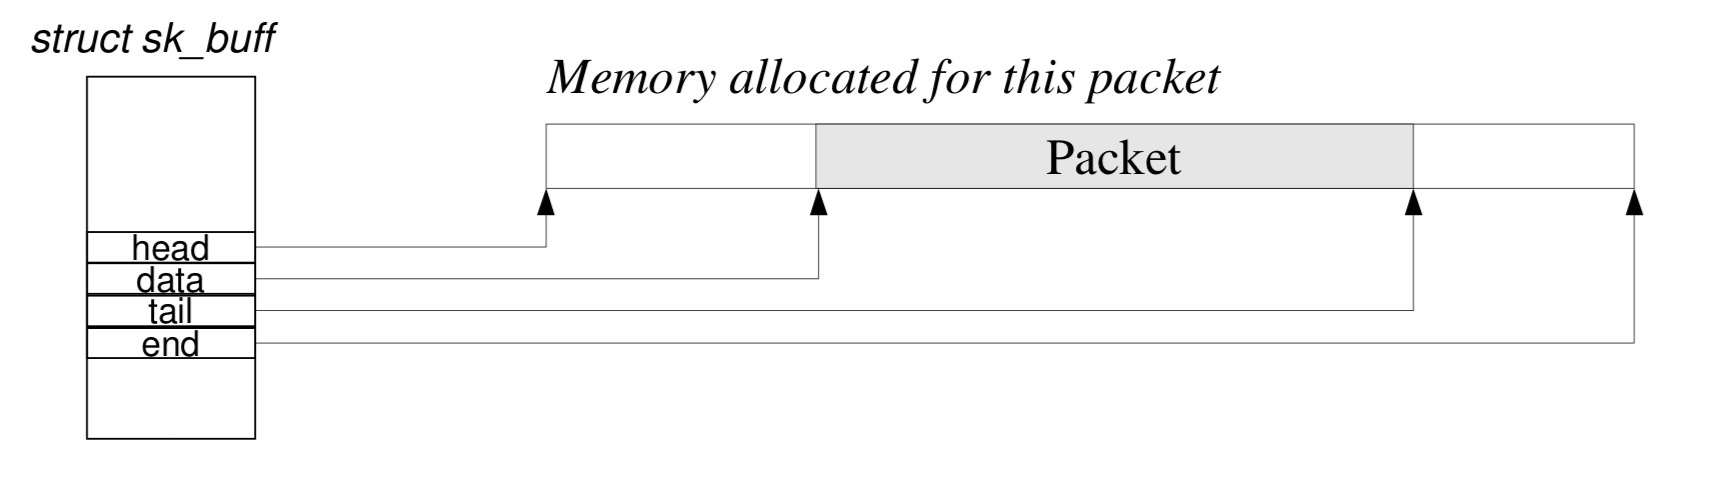
\includegraphics[width=\textwidth]{Final/skbuff.png}
       \caption{SKB Data Structure}
       \label{fig:compbest}
\end{figure}

\subsubsection{Inserting the CW Header}
The steps to add the CW header to the packet is given below.  
The commands given in the table 3.1 are various SKB operations\cite{skbuff2} used for adding a Header and the same is followed for adding CW Header

\begin{table}[htbp]
  \centering
  \caption{skbuff commands}
    \begin{tabular}{|l|p{23.39em}|}
    \toprule
    \hline
    \multicolumn{1}{|c|}{Command} & \multicolumn{1}{c|}{Action} \\
    \midrule
    \hline
    skb\_cow\_head & This command will check if there is enough headroom available in the size of max header length of CW Header \\
    \midrule
    \hline
    skb\_push & This command is used for allocating the header length space for the data structure \\
    \midrule
    \hline
    memmove & This command is used for moving the mac header to the newly allocated space so that we can insert the CW header in the place of MAC header (Between the payload and MAC header) \\
    \midrule
    \hline
    skb\_reset\_mac\_header & This command will reset the pointer to the mac header to the new location of MAC header \\
    \midrule
    \hline
    skb\_mac\_header(skb) + skb->mac\_len & This command points to the start of CW space so that the CV values can be added \\
    \hline
    \bottomrule
    \end{tabular}%
  \label{tab:addlabel}%
\end{table}%



\subsubsection{Encryption of Data}  

Encryption of data is performed by Linux Crypto API and it’s has rich set of all the cryptographic algorithms. For the best understanding of the usage of Linux Crypto APIs, we have to study a bit about the architecture specifications and functional flow of these Crypto APIs \\

There are 2 major components in the Kernel Crypto API which are called Cipher Handles and Request Handles. The Cipher Handles contains all the configurations and settings of the given type of encryption to be used and the request handler handles the encryption requests. \\

The steps to encrypt the packet are given in the Table 3.2,\\


\begin{table}[ht]
  \centering
  \caption{Linux Crypto Commands for encryption}
    \begin{tabular}{|l|l|}
    \toprule
    \hline
    \multicolumn{1}{|c|}{Command} & \multicolumn{1}{c|}{Action} \\
    \hline
    \midrule
    \multicolumn{1}{|p{15.89em}|}{Initialize ’crypto\_aead’ and ’aead\_request’} & \multicolumn{1}{p{22.5em}|}{This command is used for initialising the AEAD Cipher Handler and Request Handler} \\
    \hline
    \midrule
    crypto\_alloc\_aead & \multicolumn{1}{p{22.5em}|}{This command is used for allocating the AEAD Cipher handler} \\
    \hline
    \midrule
    aead\_request\_alloc & \multicolumn{1}{p{22.5em}|}{This command is used for allocating the AEAD Request handler} \\
    \hline
    \midrule
    aead\_request\_set\_callback & \multicolumn{1}{p{22.5em}|}{This command will set the asynchronous call back function which will be executed upon the successful encryption} \\
    \hline
    \midrule
    crypto\_aead\_setkey & \multicolumn{1}{p{22.5em}|}{This command is to set the encryption key which is already generated in the Cipher Handler} \\
    \hline
    \midrule
    aead\_request\_set\_crypt & \multicolumn{1}{p{22.5em}|}{This command will set the data buffers for the encryption process. The plain text data to be encrypted will be concatenated at the start} \\
    \hline
    \midrule
    aead\_request\_set\_ad & \multicolumn{1}{p{22.5em}|}{This command is used for Generating the authentication tag which is used for authenticating the data at the receiving side} \\
    \hline
    \midrule
    crypto\_aead\_encrypt & This command is to trigger the encryption process \\
    \hline
    \bottomrule
    \end{tabular}%
  \label{tab:addlabel}%
\end{table}%




Once the payload data is encrypted, the MEL will be pushed on top of the packet followed by the special purpose label packet and normal MPLS packet. 

\subsection{Changes at S3 (Egress Switch)}
 

When the encrypted packet arrived at S3, it pops the MPLS label at the top along with the MEL. It will check the nonce value in the CW header, and it will compare against its own counter. If both the nonce are matching, it will start the decryption process otherwise the packet will be discarded.\\

\subsubsection{Decryption of Data using Linux Crypto API}

Decryption of the payload is very similar to the encryption process. The only difference is instead of plain text, the input is cipher text which is a concatenated combination of associated data, authentication tag and the cipher text. The authentication tag is used to authenticate the data post the decryption and if there is an authentication failure, it will alert. The flag in crypto_aead_encrypt function is set to decrypt. The output of decryption will give a concatenated combination of associated data and plain text.\\

 

\subsection{Removal of CW}

Just like we added CW header to the packet by manipulation steps used in skbuff, we can pop the CW header from the packet. The SKBuff steps involved in popping the CW header from the packet is given in the Table 3.3.\\


\begin{table}[ht]
  \centering
  \caption{skbuff commands for popping a header}
    \begin{tabular}{|l|p{22.5em}|}
    \toprule
    \hline
    \multicolumn{1}{|c|}{Command} & \multicolumn{1}{c|}{Action} \\
    \hline
    \midrule
    skb\_postpull\_rcsum & This command is used for recalculating the checksum once then MEL is pulled out of the packet \\
    \hline
    \midrule
    memmove & This command is used for moving the MAC header to the place of CW \\
    \hline
    \midrule
    \_\_skb\_pull & This command will pull the size of CW Header (4 bytes) from the top of the skb data structure \\
    \hline
    \midrule
    skb\_reset\_mac\_header & This command is used shifting the MAC header pointer to the new position of the MAC header \\
    \hline
    \midrule
    skb\_set\_network\_header & This command is used for setting the network header pointer to the position of the new network header \\
    \hline
    \bottomrule
    \end{tabular}%
  \label{tab:addlabel}%
\end{table}%




\section{Testing the MPLS OS System}
Once the Opportunistic Security is implemented in the OVS code, we have to compile the OVS kernel. All the kernel files of the OVS is kept in the folder called datapath and the majority of the changes are performed in the file called action.c. The header files are kept under linux/compat/include/net. The OVS have a makefile which is used for the compilation. Once the compilation is done if we have previously installed OVS in the Linux kernel, we have to remove is by rmmod or modprobe. A simple ’rmmod openvswitch’ will remove the openvswitch from the linux kernel. Make sure to stop the openvswitch before compiling the code. Detailed building, compiling and loading steps of openvswitch is submitted in the git repository of the research report. Once the compilation is done, we can load the openvswith to the linux kernel using modprobe,  ’modprobe openvswitch’. We can check if we correctly loaded the openvswitch in the kernel by using lsmod.

\subsection{Addition of the MPLS OS flows}

The difference between the flows of traditional MPLS and MPLS OS is the addition of Special Purpose Label, the CW and the MEL. These header additions are not performed by the OpenFlow Flow because there is only very limited packet modifications are possible in OpenFlow such as changing the ether type. These headers are added only when a packet is send encrypted which is only happen by end of a successful key exchange between the participating LSRs. As discussed above there are 3 MPLS labels are added in MPLS OS such as the MEL with value 1, the special purpose label with label value 15 and another MPLS label for routing. The issue encountered during the development is that packet was discarded at S3 without sending to the destination host and the reason was the OVS cannot pop multiple labels of the same packet and the OVSK was forwarding the packet to userspace\cite{OVSMail2}E. This issue has to be fixed by OVS and meantime the workaround adapted is that instead of pushing 3 Labels, push a single label with value 1and this label will act as the functional combination of all 3 labels proposed in the design.\\

With the workaround the modified MPLS FLow is as given below,\\

sudo ovs-ofctl -O OpenFlow13 add-flow s1 "table=0,in_port=1,eth_type=0x800,actions=goto_table:1" 

sudo ovs-ofctl -O OpenFlow13 add-flow s1 "table=1,in_port=1,eth_type=0x800,actions=push_mpls:0x8847,set_field:1->mpls_label,output:2" 

sudo ovs-ofctl -O OpenFlow13 add-flow s2 "table=0,in_port=2,eth_type=0x8847,actions=output:3" 

sudo ovs-ofctl -O OpenFlow13 add-flow s3 "table=0,in_port=2,eth_type=0x8847,actions=goto_table:1" 

sudo ovs-ofctl -O OpenFlow13 add-flow s3 "table=1,in_port=2,eth_type=0x8847,mpls_label=1,mpls_bos=1,actions=pop_mpls:0x800,output:1" \\

 

sudo ovs-ofctl -O OpenFlow13 add-flow s3 "table=0,in_port=1,eth_type=0x800,actions=goto_table:1" 

sudo ovs-ofctl -O OpenFlow13 add-flow s3 "table=1,in_port=1,eth_type=0x800,actions=push_mpls:0x8847,set_field:1->mpls_label,output:2" 

sudo ovs-ofctl -O OpenFlow13 add-flow s2 "table=0,in_port=3,eth_type=0x8847,actions=output:2" 

sudo ovs-ofctl -O OpenFlow13 add-flow s1 "table=0,in_port=2,eth_type=0x8847,actions=goto_table:1" 

sudo ovs-ofctl -O OpenFlow13 add-flow s1 "table=1,in_port=2,eth_type=0x8847,mpls_label=1,mpls_bos=1,actions=pop_mpls:0x800,output:1" \\

 

sudo ovs-ofctl -O OpenFlow13 add-flow s1 "table=0,in_port=1,eth_type=0x806,actions=output:2" 

sudo ovs-ofctl -O OpenFlow13 add-flow s1 "table=0,in_port=2,eth_type=0x806,actions=output:1" 

sudo ovs-ofctl -O OpenFlow13 add-flow s2 "table=0,in_port=2,eth_type=0x806,actions=output:3" 

sudo ovs-ofctl -O OpenFlow13 add-flow s2 "table=0,in_port=3,eth_type=0x806,actions=output:2" 

sudo ovs-ofctl -O OpenFlow13 add-flow s3 "table=0,in_port=1,eth_type=0x806,actions=output:2" 

sudo ovs-ofctl -O OpenFlow13 add-flow s3 "table=0,in_port=2,eth_type=0x806,actions=output:1" 

\subsection{Testing Communication for MPLS with OS}

MPLSOS works very similar to traditional MPLS. The difference is that the packets between 2 participating LSRs are encrypted.The key for encryption and decryption is generated after a DH Key exchange. The very first packet send between 2 participating LSRs (S1 and S3 in the experiment setup) is a DH Key exchange which is in plain text and there will be an MPLS TLV\cite{__2017}\cite{__2014}\cite{___2009} between the MPLS header and Ethernet Header.

\begin{figure}[ht]
       \centering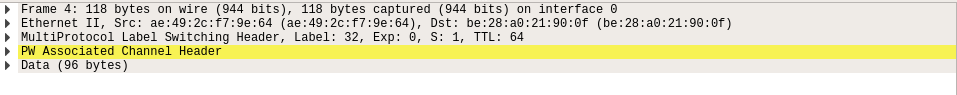
\includegraphics[width=\textwidth]{Final/MPLS_TLV.png}
       \caption{MPLS TLV}
       \label{fig:compbest}
\end{figure}

This TLV will have the DH Group, DH Key, Encryption Algorithm etc and the receiving LSR can calculate the shared secret key for encryption and decryption.\\

Once the key is generated, the very packet onwards the LSR will start encrypting using the key generated. In the experiment setup the host H1 will send plaintext ICMP Ping to Host H3. The packet will arrive Switch S1 which is a participating LSR and S1 encrypt the packet, then add MEL and CW, then send to S3 through S2. S3 will pop the MEL and CW, then decrypt the packet and forward the plain ICMP packet to H3. ICMP Reply from H3 to H1 will follow the reverse path of the request packet.


\begin{figure}[ht]
       \centering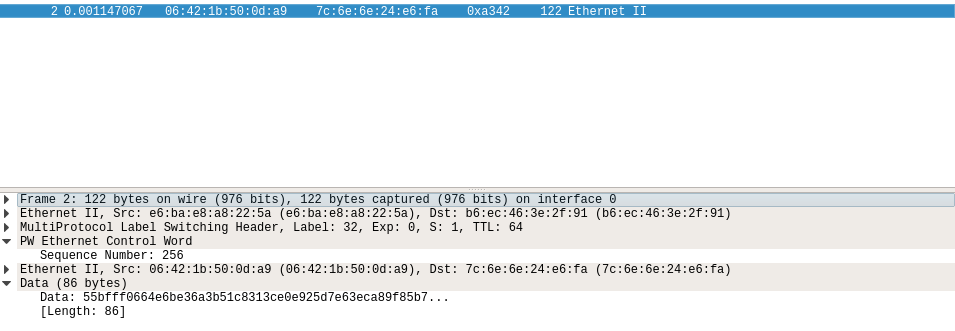
\includegraphics[width=\textwidth]{Final/MPLSOS_Working.png}
       \caption{MPLSOS Packet}
       \label{fig:compbest}
\end{figure}
